\chapter{Spring Data JPA Transaction management}

\fcolorbox{black}[HTML]{E9F0E9}{\parbox{\textwidth}{%
\noindent \textbf{Learning goals}\\
The junior-colleague
\begin{enumerate}[nolistsep]
\item can explain the ACID-properties of a transaction.
\item can implement transactions in spring boot applications.
\item can explain what a connection pool is.
\item can explain what transaction propagation is.
\item can explain the different possible transaction propagation methods.
\item can explain different isolation levels and the problems that can possibly occur.
\item can use flyway to implement database migrations.
\end{enumerate}}}

\section{Introduction}

A database transaction is a sequence of actions that are treated as a single unit of work. The actions should either complete entirely or take no effect at all. Transaction management is an important part of RDBMS-oriented enterprise application to ensure data integrity and consistency. The concept of transactions can be described with the following four key properties described as ACID \footnote{\url{https://www.youtube.com/watch?v=VRm2UMsFVz0}}:

\begin{itemize}
\item \textbf{Atomicity} A transaction should be treated as a single unit of operation, which means either the entire sequence of operations is successful or unsuccessful.

\item \textbf{Consistency} This represents the consistency of the referential integrity of the database, unique primary keys in tables, etc.

\item \textbf{Isolation} There may be many transaction processing with the same data set at the same time. Each transaction should be isolated from others to prevent data corruption.

\item \textbf{Durability} Once a transaction has completed, the results of this transaction have to be made permanent and cannot be erased from the database due to system failure.
\end{itemize}

If you are using a Spring Boot project and have a spring-data-* dependency on the classpath, then transaction management is enabled by default.

\section{Hikari connection pool}

\begin{verbatim}
HikariPool-1 - Starting...
HikariPool-1 - Added connection org.mariadb.jdbc.Connection@479111ba
HikariPool-1 - Start completed.
\end{verbatim}

Connection Pooling (CP) is the way to keep database connections open so that they can be reused by other clients (repositories), in other words, it is cache of database connections reused when future request to database is required. The application can access data at a faster rate, thereby reducing the number of database connections.
The default connection pool for Spring Boot applications is the Hikari Connection Pool (HikariCP).
Hikari-specific settings can be defined in the application.yml or application.properties file.

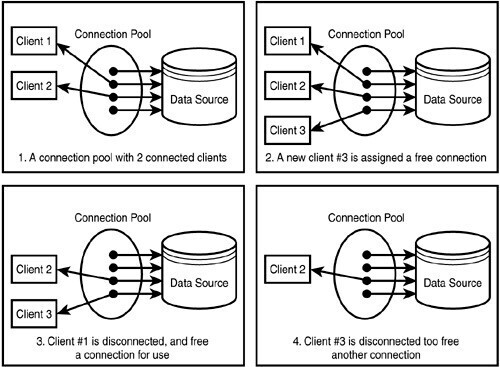
\includegraphics[width=\textwidth]{./images/chapter-tx/connection_pool.jpg}

\section{Transactions}

In most SpringBoot applications you will find two @Transactional annotations. One is provided by Spring the other is provided by JTA(Jakarta Transactional Annotations). They are in different packages. So when using the annotation make sure you know which one you have imported. We recommend using the one provided by Spring.

Just by using that annotation Spring does all the magic and we will not even be aware of what has happened.
You can always add the following properties to log the creation, commit and rollback of transactions.

\begin{verbatim}
logging.level.org.springframework.transaction.interceptor=trace
logging.level.org.springframework.orm.jpa=debug
logging.level.org.springframework.transaction=debug
\end{verbatim}

The @Transactional annotation is convenient because we as developers no longer need to think about how to start a transaction, how to execute it and when to do rollback or commit.

All of this is done automatically in a proxy class that Spring creates to hold the transaction management code. So yes, all those boilerplate codes are there but we just don’t see it. At run time, when the method annotated with @Transactional is called Spring, create a proxy class, in that proxy class it writes all the necessary codes to manage the transaction then it calls the actual class. to the logic and codes related to transactions is only done in the proxy class.

In its default configuration, the Spring Framework’s transaction infrastructure code marks a transaction for rollback only in the case of runtime, unchecked exceptions. That is, when the thrown exception is an instance or subclass of RuntimeException. (Error instances also, by default, result in a rollback). Checked exceptions that are thrown from a transactional method do not result in rollback in the default configuration.

\section{Transaction propagation}


Transaction propagation is the behavior of a transaction from one class to another. This means if class A has a method that creates a transaction and that method at some point has to call another transactional method in class B how should be the behavior of the method class B in regard to the transaction started by class A. And if there was no transaction started by class A what would class B do about that?

The possible transaction propagation methods are:

\begin{itemize}
\item \textbf{REQUIRED} This is the default propagation option. If a transaction already exists when a method annotated with REQUIRED is called, the method will execute within that transaction. If no transaction exists, a new transaction will be started.

\item \textbf{REQUIRES\_NEW} This option always starts a new transaction, even if a transaction already exists.

\item \textbf{SUPPORTS} This option allows a method to participate in a transaction if one already exists, but doesn’t start a new transaction if one doesn’t exist.

\item \textbf{MANDATORY} This option requires that a transaction already exists. If a transaction doesn’t exist, an exception is thrown.

\item \textbf{NOT\_SUPPORTED} This option specifies that a method should not participate in a transaction at all.

\item \textbf{NEVER} This option specifies that a method should never be called within a transaction.
\end{itemize}

More information: \url{https://dzone.com/articles/spring-transaction-propagation}

\url{https://www.geeksforgeeks.org/spring-boot-transaction-management-using-transactional-annotation/}

\section{Transaction isolation level}

Isolation determines how transaction integrity is visible to other users and systems.
Isolation levels define the degree to which a transaction must be isolated from the data modifications made by any other transaction in the database system. A transaction isolation level is defined by presence or absence of the following concurrency issues. 

\subsection{Concurrency Issues}

\subsubsection{Dirty Read}

A transaction reads the data that has not been committed by another transaction.

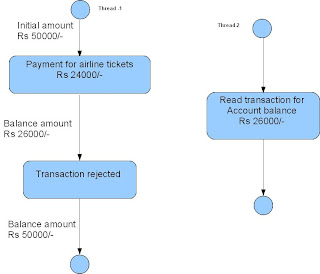
\includegraphics{./images/chapter-tx/DirtyRead.JPG}

\subsubsection{Lost Updates}

A lost update problem occurs due to the update of the same record by two different transactions at the same time. In simple words, when two transactions are updating the same record at the same time then a lost update problem occurs.

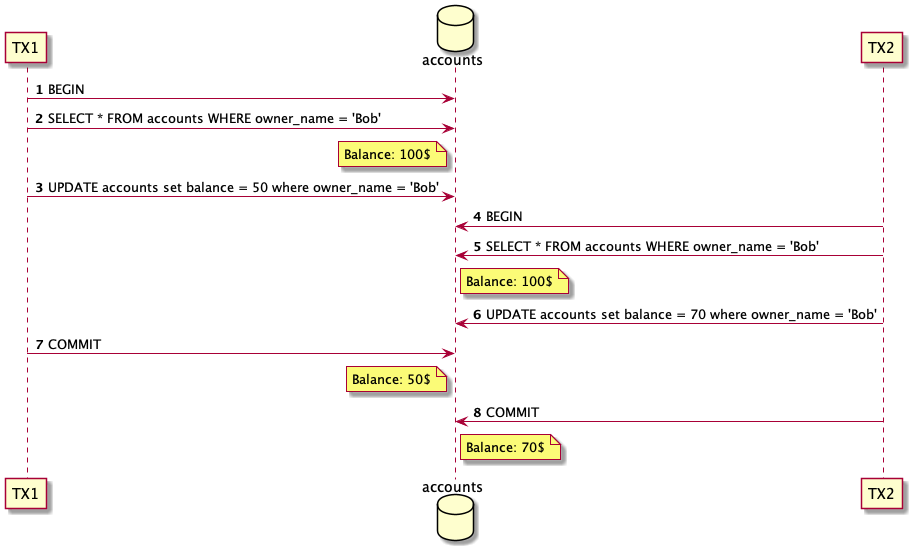
\includegraphics[width=\textwidth]{./images/chapter-tx/lost_update.png}

\subsubsection{Nonrepeatable Read}

Transaction reads the same row more than once and another transaction changes the data in the row between the successive reads of the transaction.

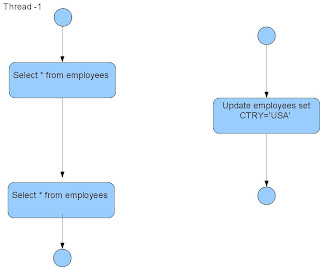
\includegraphics{./images/chapter-tx/NonRepeatable.JPG}

\subsubsection{Phantom Read}

A transaction reads a rowset more than once and another transaction inserts or deletes a row between the successive reads.

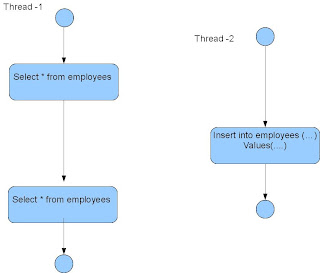
\includegraphics{./images/chapter-tx/PhantomRead.JPG}

\subsection{Setting Transaction Isolation Levels}

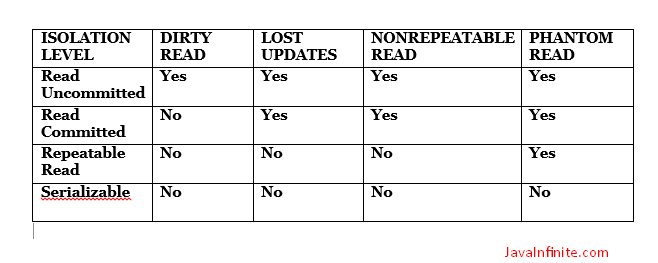
\includegraphics{./images/chapter-tx/isolation_level.png}

Isolation levels define the degree to which a transaction must be isolated from the data modifications made by any other transaction in the database system. 
Transaction isolation levels can improve concurrency by allowing multiple transactions to run concurrently without interfering with each other.


\subsubsection{Read Uncommitted}
In this level, a transaction can read the data modified by another transaction. But a transaction can read the data modified by another transaction even before the commit is made. Dirty Reads, Lost Updates, Nonrepeatable Read and Phantom read all issues occur at this level.

\subsubsection{Read Committed}
This is the default Isolation level in SQL database. In this level, When a transaction modifies a data other transactions will not be able to read the modified data. This prevents Dirty Reads but Lost Updates, Nonrepeatable Read and Phantom Read occurs at this level.

\subsubsection{Repeatable Read}
In this level, when a transaction is modifying data, no other transactions can read or ypdate the data until the current transaction completes it process. At this level, Dirty Reads, Lost Updates and Nonrepeatable Read are prevented but Phantom Read may occur.

\subsubsection{Serializable}
In this level, when a transaction is modifying data, no other transaction can read, update, modify or insert data until the current transaction completes its process and commits.


The default isolation level for Spring Boot application will be the default isolation of the RDBMS. MySQL and MariaDB's default isolation level is `Repeatable Read'. On the other hand, PostgreSQL and Oracle is `Read Committed'.


\section{Flyway}

Flyway is an open-source library used for Database Migration / Version Control for the DB scripts. It allows us to migrate the changes to DB incrementally by versioning.
Spring Boot provides easy integration with Flyway.


\begin{verbatim}
<dependency>
    <groupId>org.flywaydb</groupId>
    <artifactId>flyway-core</artifactId>
</dependency>
<dependency>
    <groupId>org.flywaydb</groupId>
    <artifactId>flyway-mysql</artifactId>
</dependency>
\end{verbatim}

The database migration are written in sql scripts. Make sure you follow the naming convention, otherwise the script will not be executed.

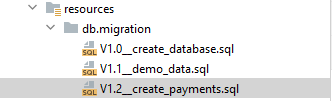
\includegraphics{./images/chapter-tx/flyway2.png}

Flyway creates a table flyway\_schema\_history where the current status of the database can be found.

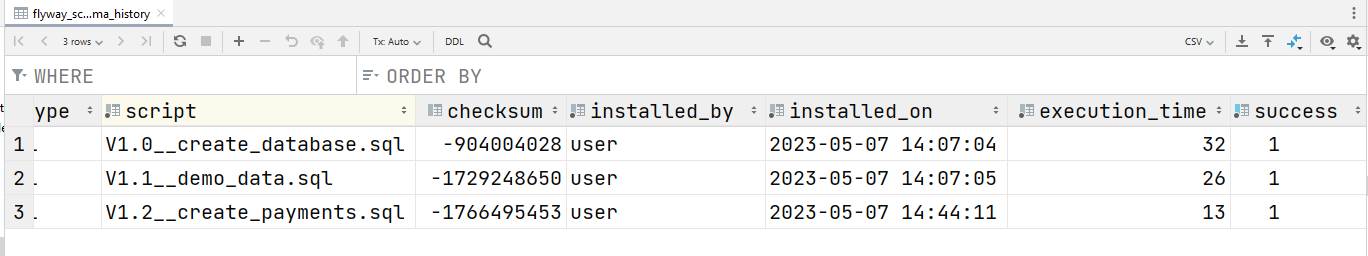
\includegraphics[width=\textwidth]{./images/chapter-tx/flyway1.png}

An alternative for flyway is liquibase.





